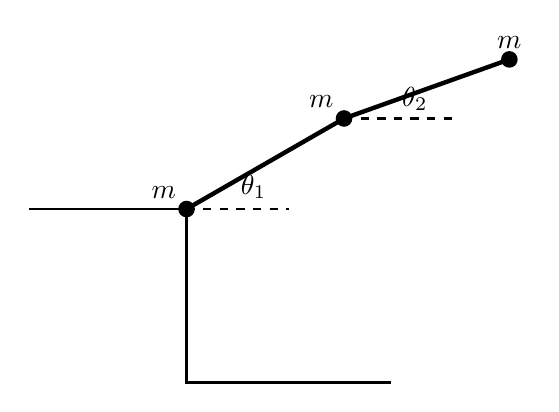
\begin{tikzpicture}[line width=1pt]
\coordinate (P1) at (0,0);
\coordinate (P2) at (2,1.15);
\coordinate (P3) at (4.1,1.9);
\draw (-2,0) -- (P1);
\draw (P1) -- (0,-2.2) -- (2.6,-2.2);
\draw[line width=1.6pt] (P1) -- (P2) -- (P3);
\fill (P1) circle (3pt); \fill (P2) circle (3pt); \fill (P3) circle (3pt);
\node[above left] at (P1) {$m$};
\node[above left] at (P2) {$m$};
\node[above] at (P3) {$m$};
\draw[dashed] (P1) -- (1.3,0);
\draw[dashed] (P2) -- (3.4,1.15);
\node at (0.85,0.28) {$\theta_1$};
\node at (2.9,1.4) {$\theta_2$};
\end{tikzpicture}
